% !TEX root = ../report.tex
\section{Das Partikelsystem}
\begin{Spacing}{\mylinespace}

Nachdem wir im ersten Projektsemester mit unserem CPU-basierten Partikelsystem sehr schnell an die Grenzen des machbaren gestoßen waren, haben wir uns im zweiten Projektsemester kurzfristig dafür entschieden, das System noch einmal komplett zu überarbeiten und dieses Mal auf eine reine GPU Implementierung zu setzen.

\subsection{Die Anforderungen}

Als Anforderungen haben wir uns gesetzt, ein hoch flexibles und vom restlichen System getrenntes Partikelsystem zu entwickeln, welches die Fähigkeit bietet mehrere hunderttausend oder sogar Millionen von Partikeln in Echtzeit darzustellen.  

\subsection{Die Umsetzung}
Wie bereits im Kapitel der Datencontainer kurz ansgesprochen, besteht unser Partikelsystem aus verschiedenen Texturen (Rendertargets).
Manipuliert man nun eine dieser Texturen kommt es zu einem Konflikt, denn es werden die Texturen gleichzeitig manipuliert während sie dargestellt werden.
Um dennoch eine flüssige und fehlerfreie Darstellung zu erreichen dupliziert man die Texturen und manipuliert immer nur die Texturen die gerade nicht für die Visualisierung benötigt werden.
\begin{figure}[h!]
	\centering
	\vspace*{30px}
	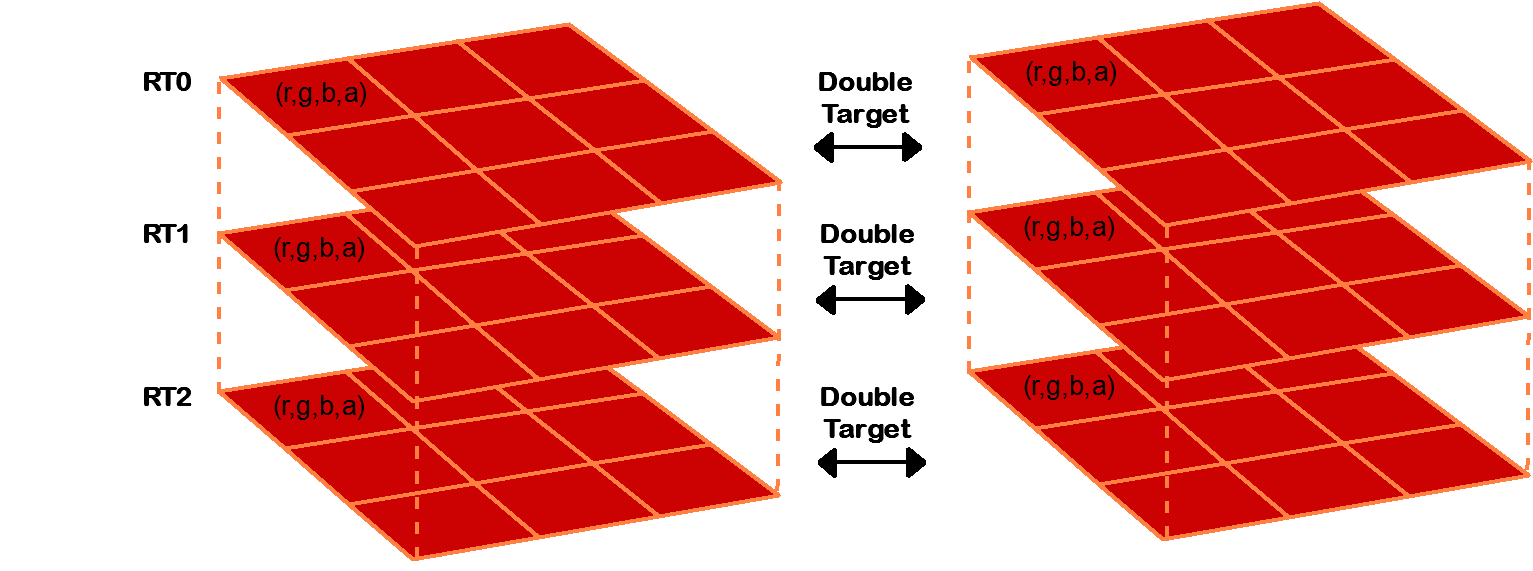
\includegraphics[width=410px]{graphics/DoubleTargets2.png}
	\caption{Double Rendertargets.}
	\label{fig:RTCahnnels}
\end{figure}
Durch die Duplizierung ist es nun einfach den beschriebenen Konflikt zu umgehen. Nachdem das erste Set der Rendertargets geupdatet wurde, wechselt man für die Aktualsierung einfach auf zweite Set (Swapping). Währenddessen kann die Visualisierung unabhängig auf dem anderen Set arbeiten ohne das Bildstörungen hervorzerufen werden.

\begin{figure}[h!]
	\centering
	\vspace*{30px}
	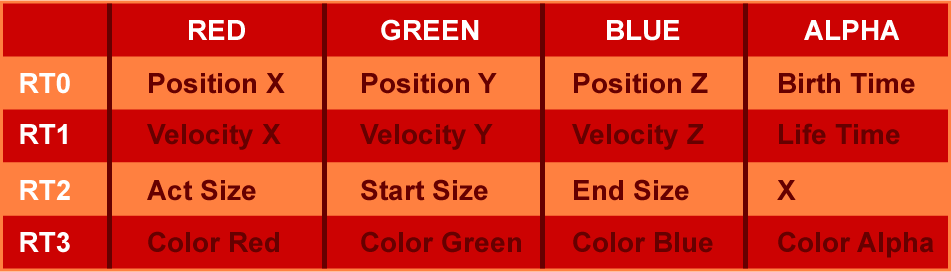
\includegraphics[width=410px]{graphics/RendertargetsChannels.png}
	\caption{Kanalbelegung der einzelnen Rendertargets.}
	\label{fig:RTCahnnels}
\end{figure}

\end{Spacing}
\newpage
\clearpage
%% End Of Doc